%\setcounter{secnumdepth}{-1}
% \chapter{Tables}\label{chap:App}

\chapter{Figures}\label{chap:App2}

\begin{figure}[h]
    \centering
 \begin{subfigure}[b]{0.49\textwidth}
     \centering
     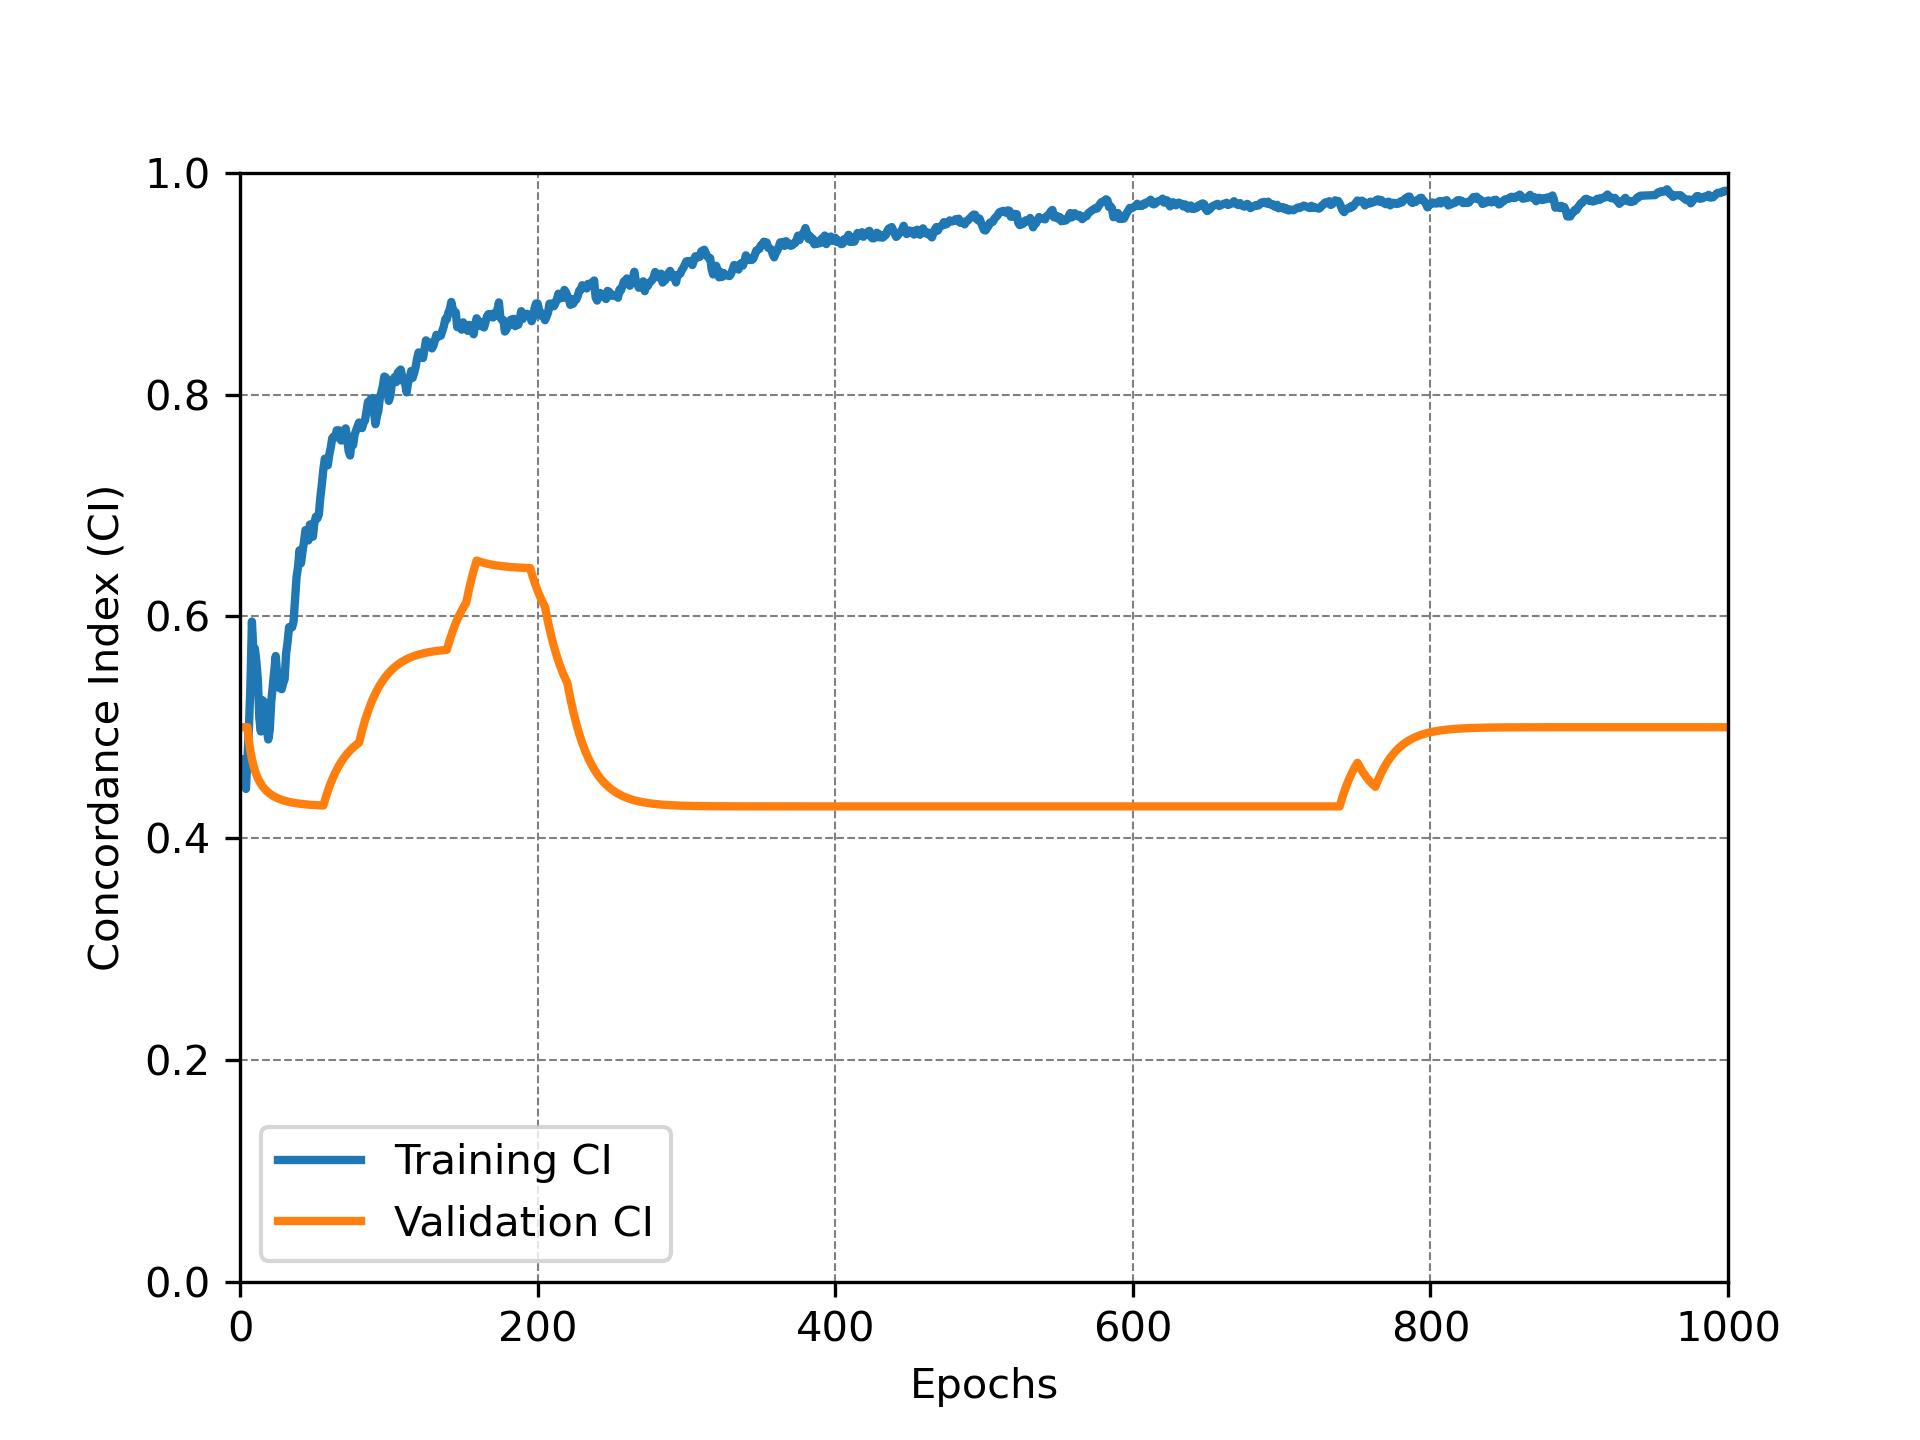
\includegraphics[width=\textwidth]{latex/ci_plots/SNNet_fsz250_1Layer.png}
     \caption{SNN with single hidden layer}
 \end{subfigure}
    \hfill
     \begin{subfigure}[b]{0.49\textwidth}
         \centering
         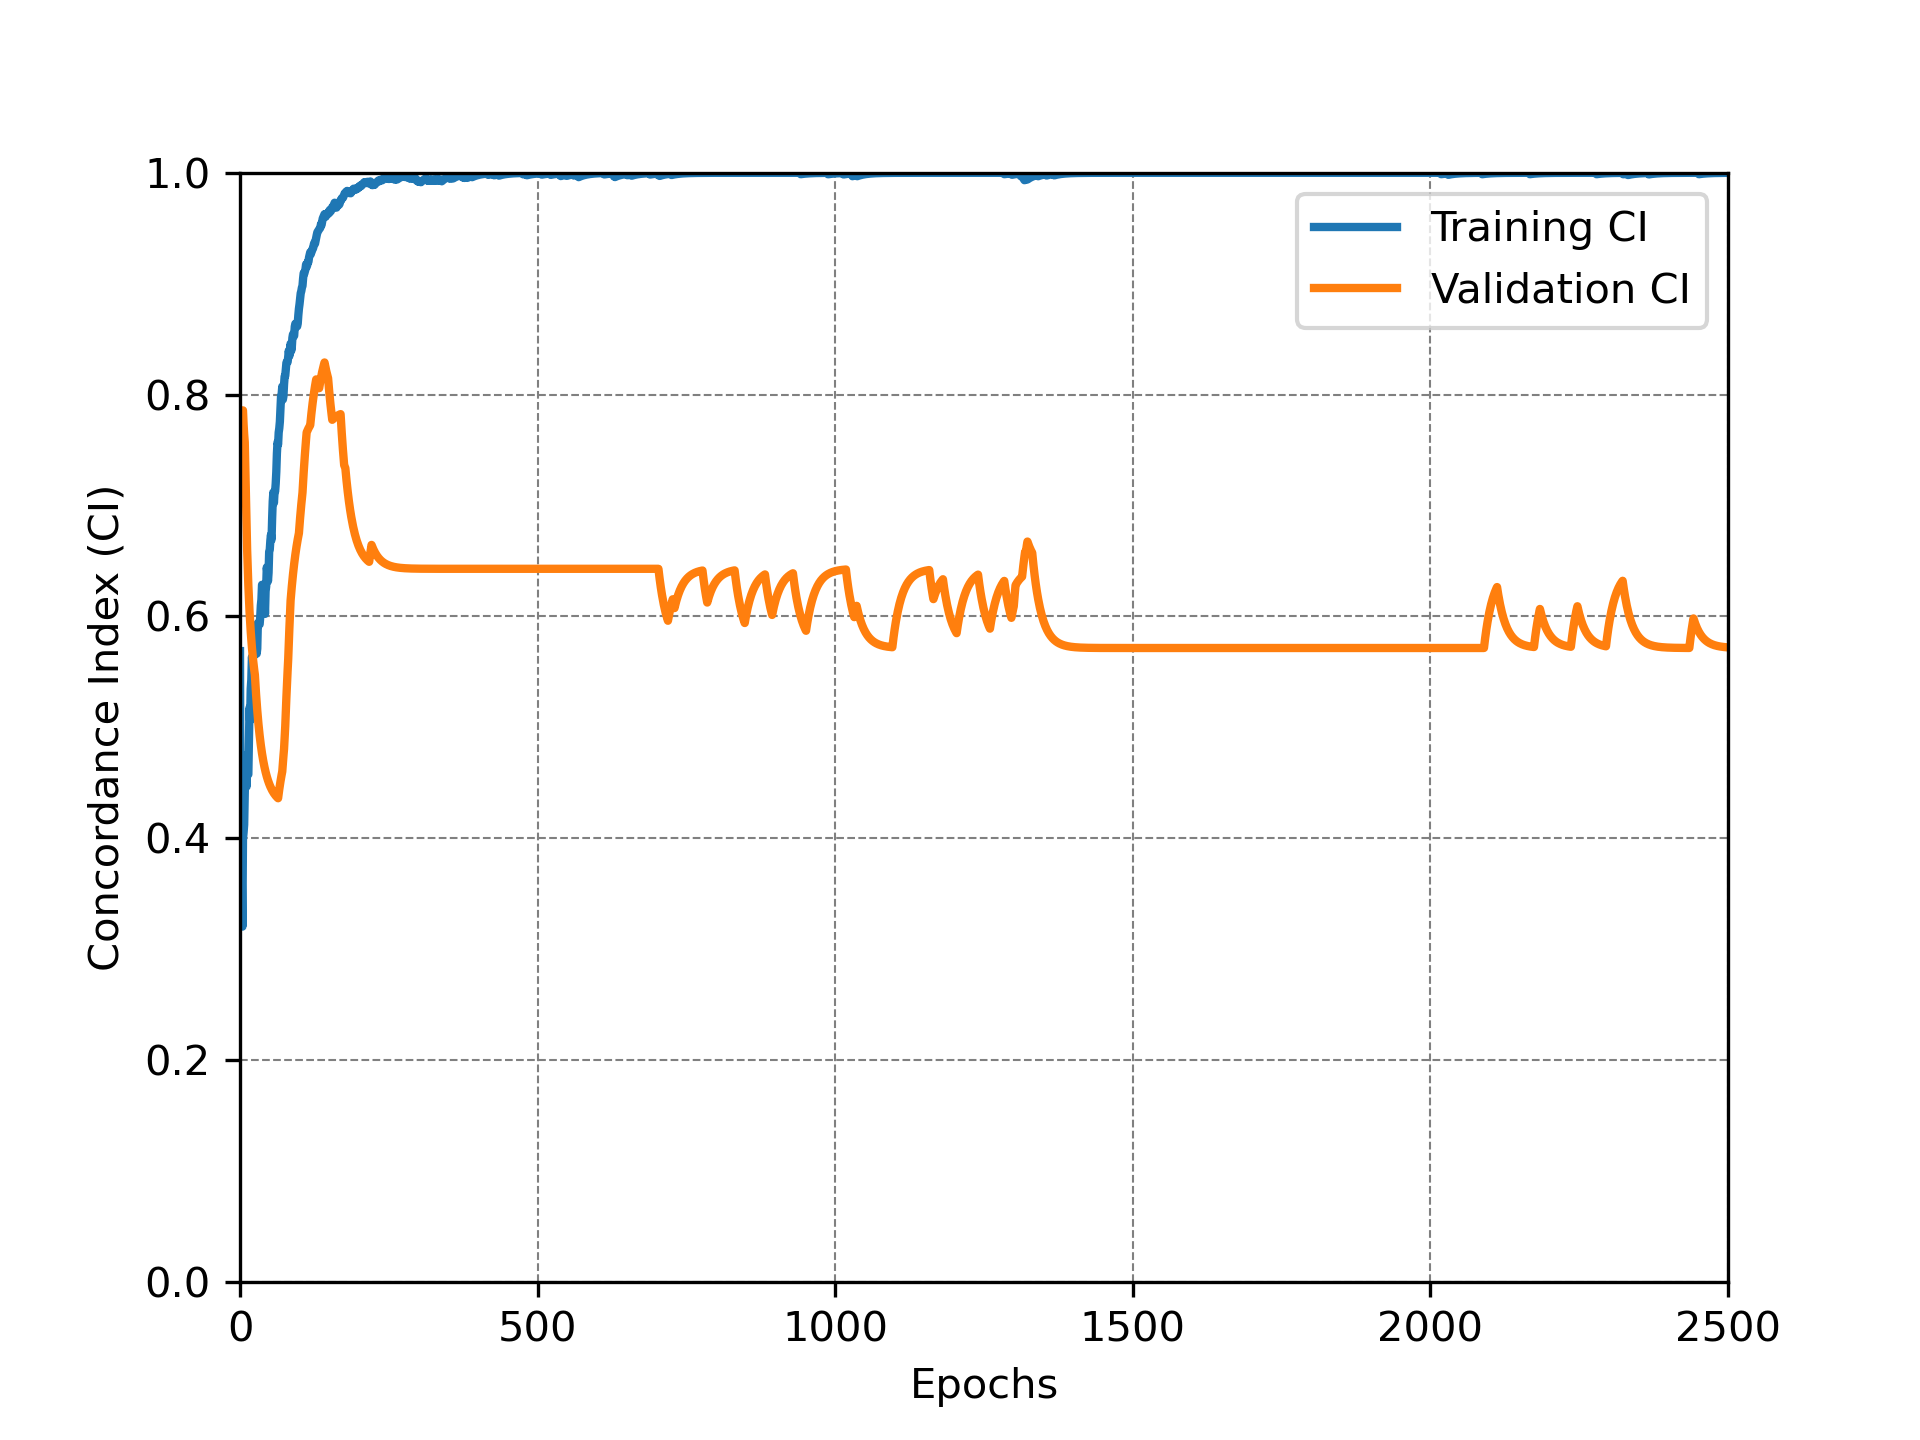
\includegraphics[width=\textwidth]{latex/ci_plots/SNNet_fsz250_1e-4_2500epochs.png}
         \caption{SNN at lr 1e-4}
     \end{subfigure}
\vskip\baselineskip
     \begin{subfigure}[b]{0.49\textwidth}
         \centering
         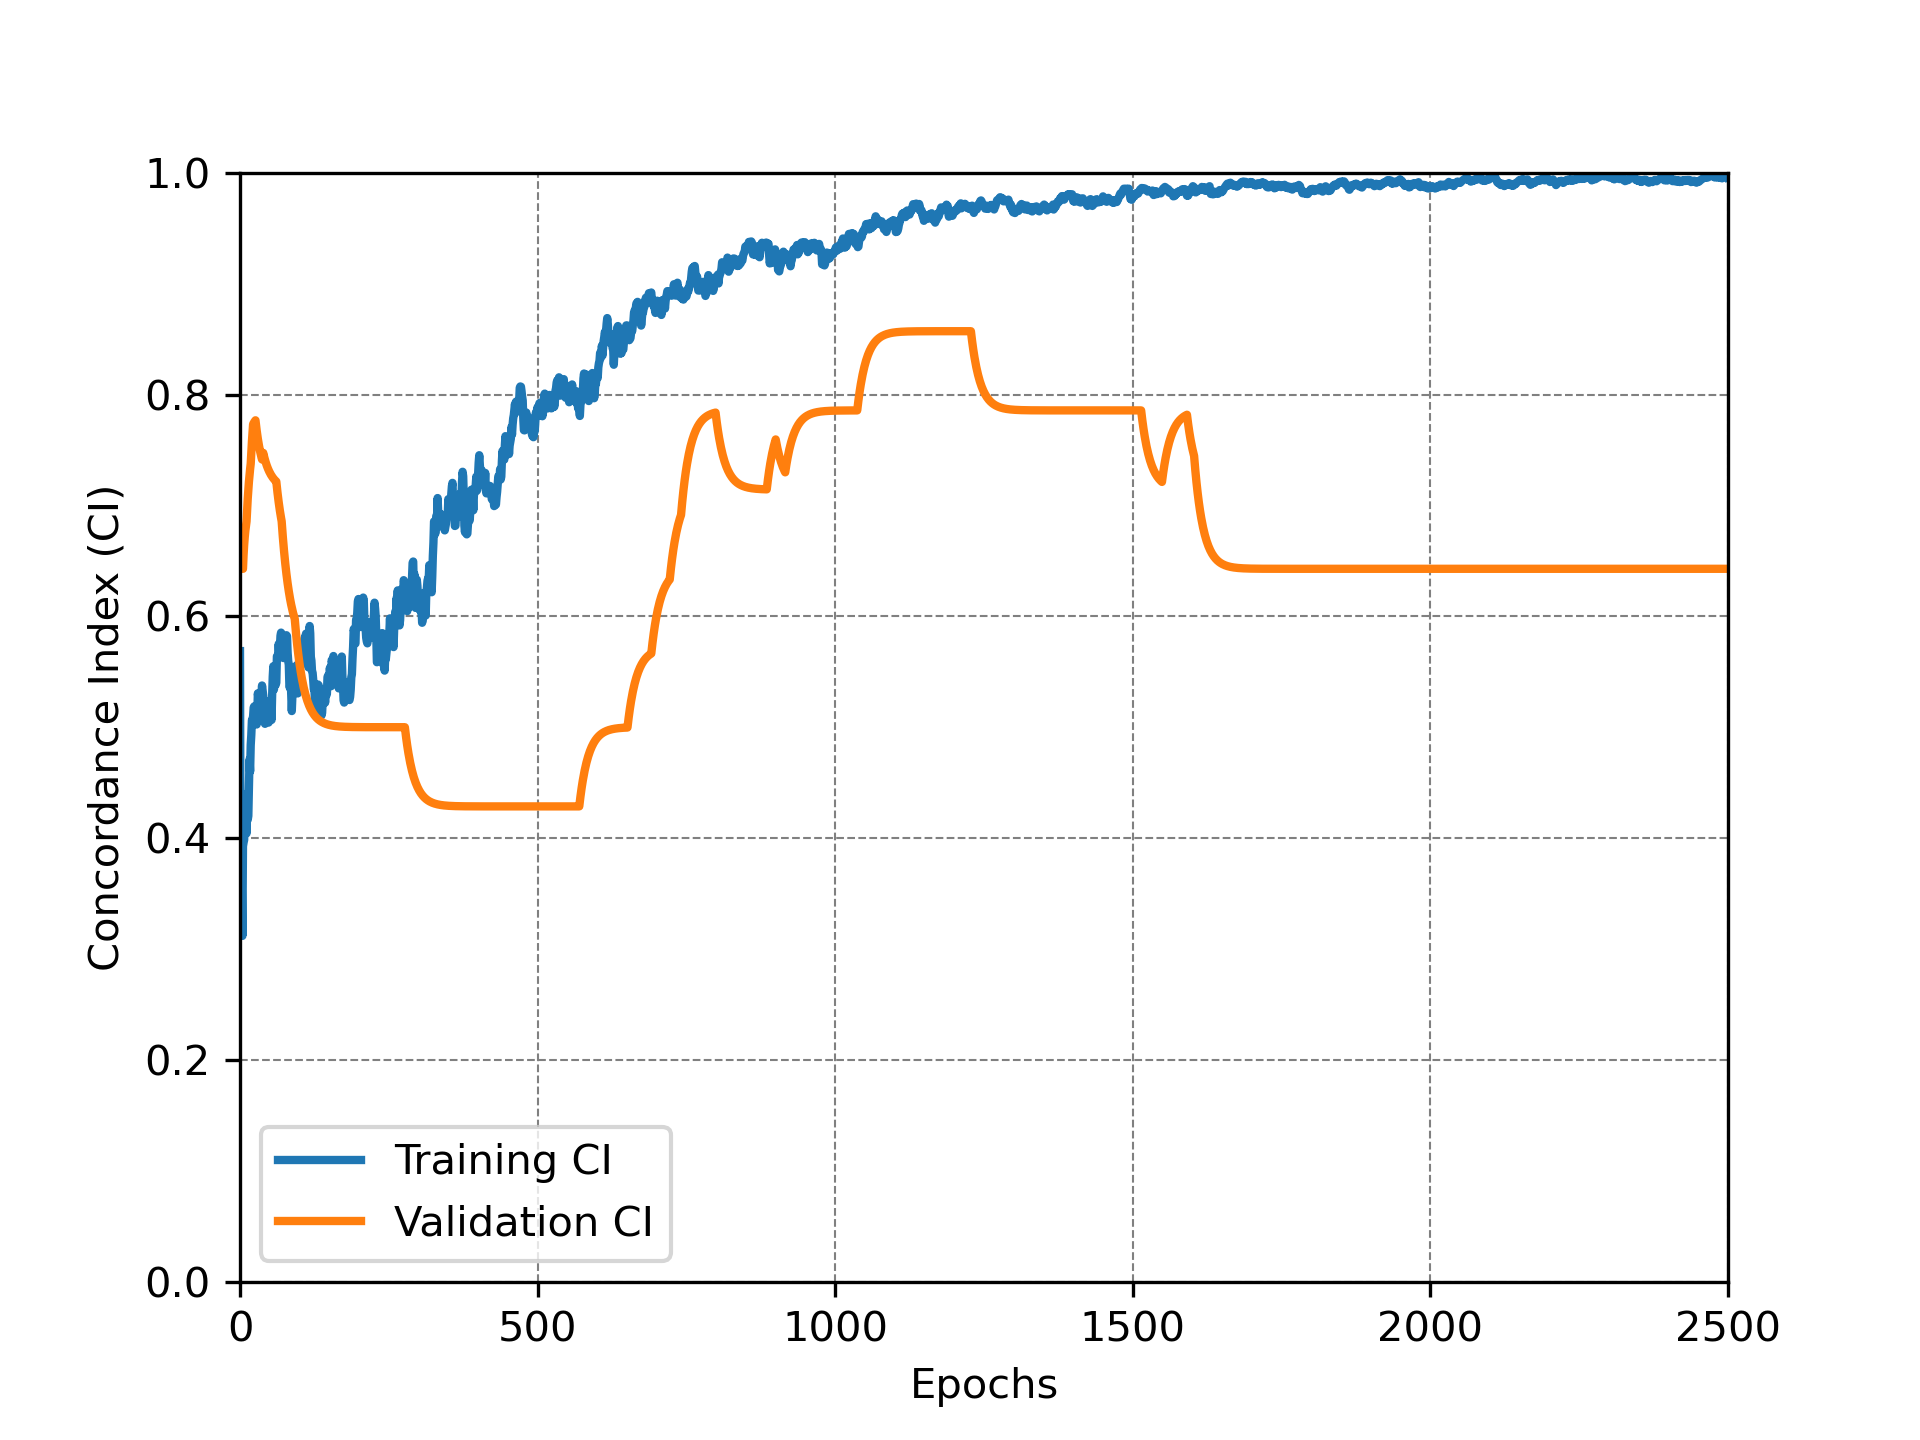
\includegraphics[width=\textwidth]{latex/ci_plots/SNNet_fsz250_1e-5_2500epochs.png}
         \caption{SNN at lr 1e-5}
     \end{subfigure}
    \hfill
     \begin{subfigure}[b]{0.49\textwidth}
         \centering
         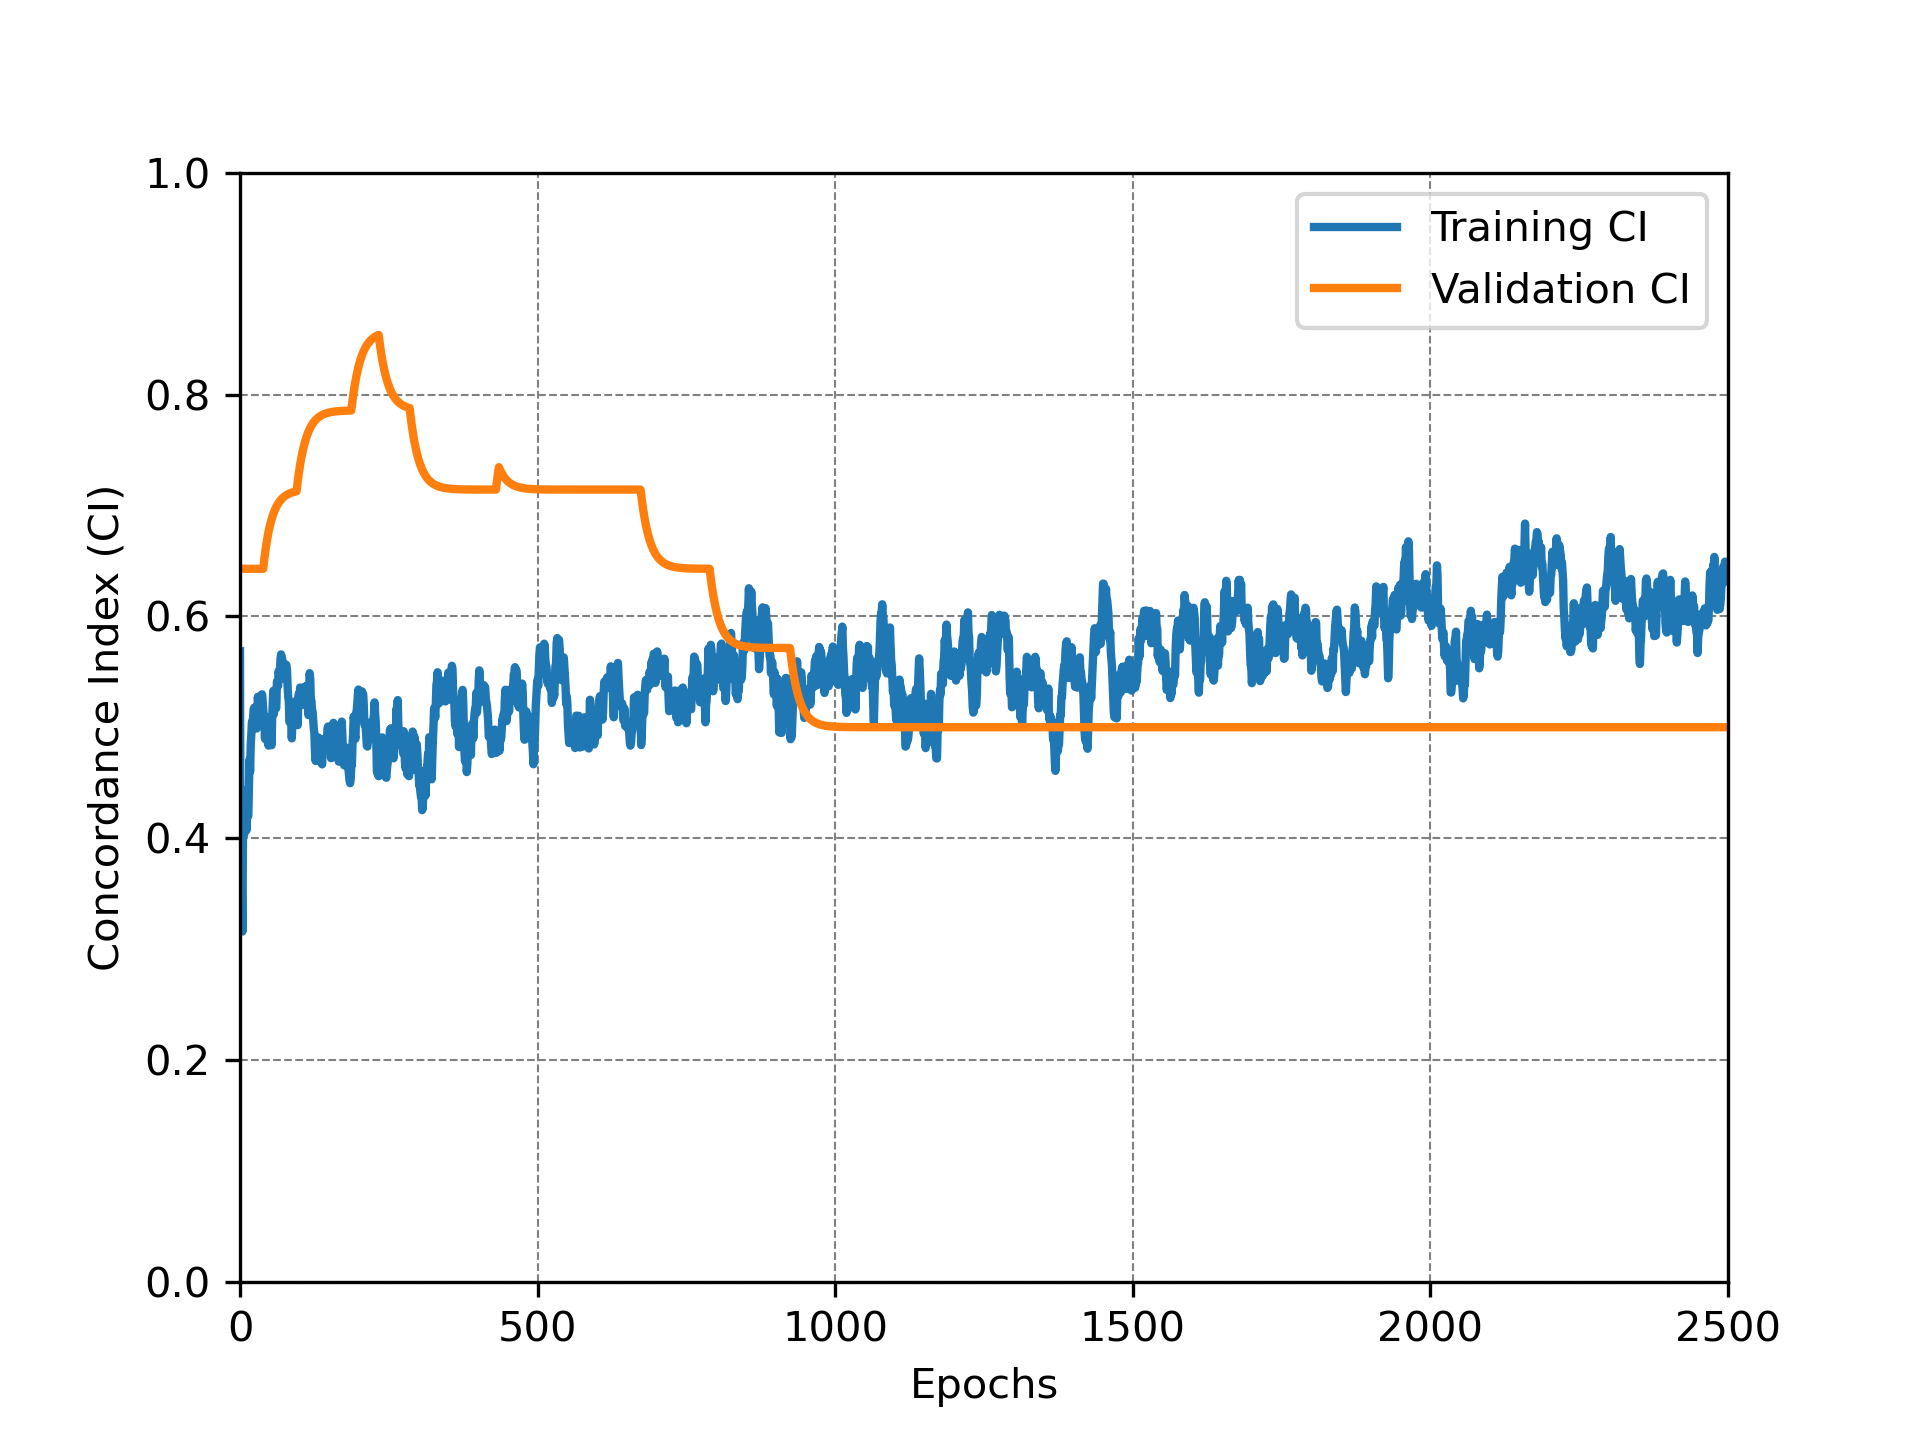
\includegraphics[width=\textwidth]{latex/ci_plots/SNNet_fsz250_1e-6_2500epochs.png}
         \caption{SNN at lr 1e-6}
     \end{subfigure}
    \hfill
    \caption[SNN with varying learning rates and models]{Experiments for SNN on learning rates and number of hidden dimensions. Neither x-axis nor y-axis are uniform.}
    \label{fig:snn_lr_ci}
\end{figure}

\begin{figure}
    \centering
    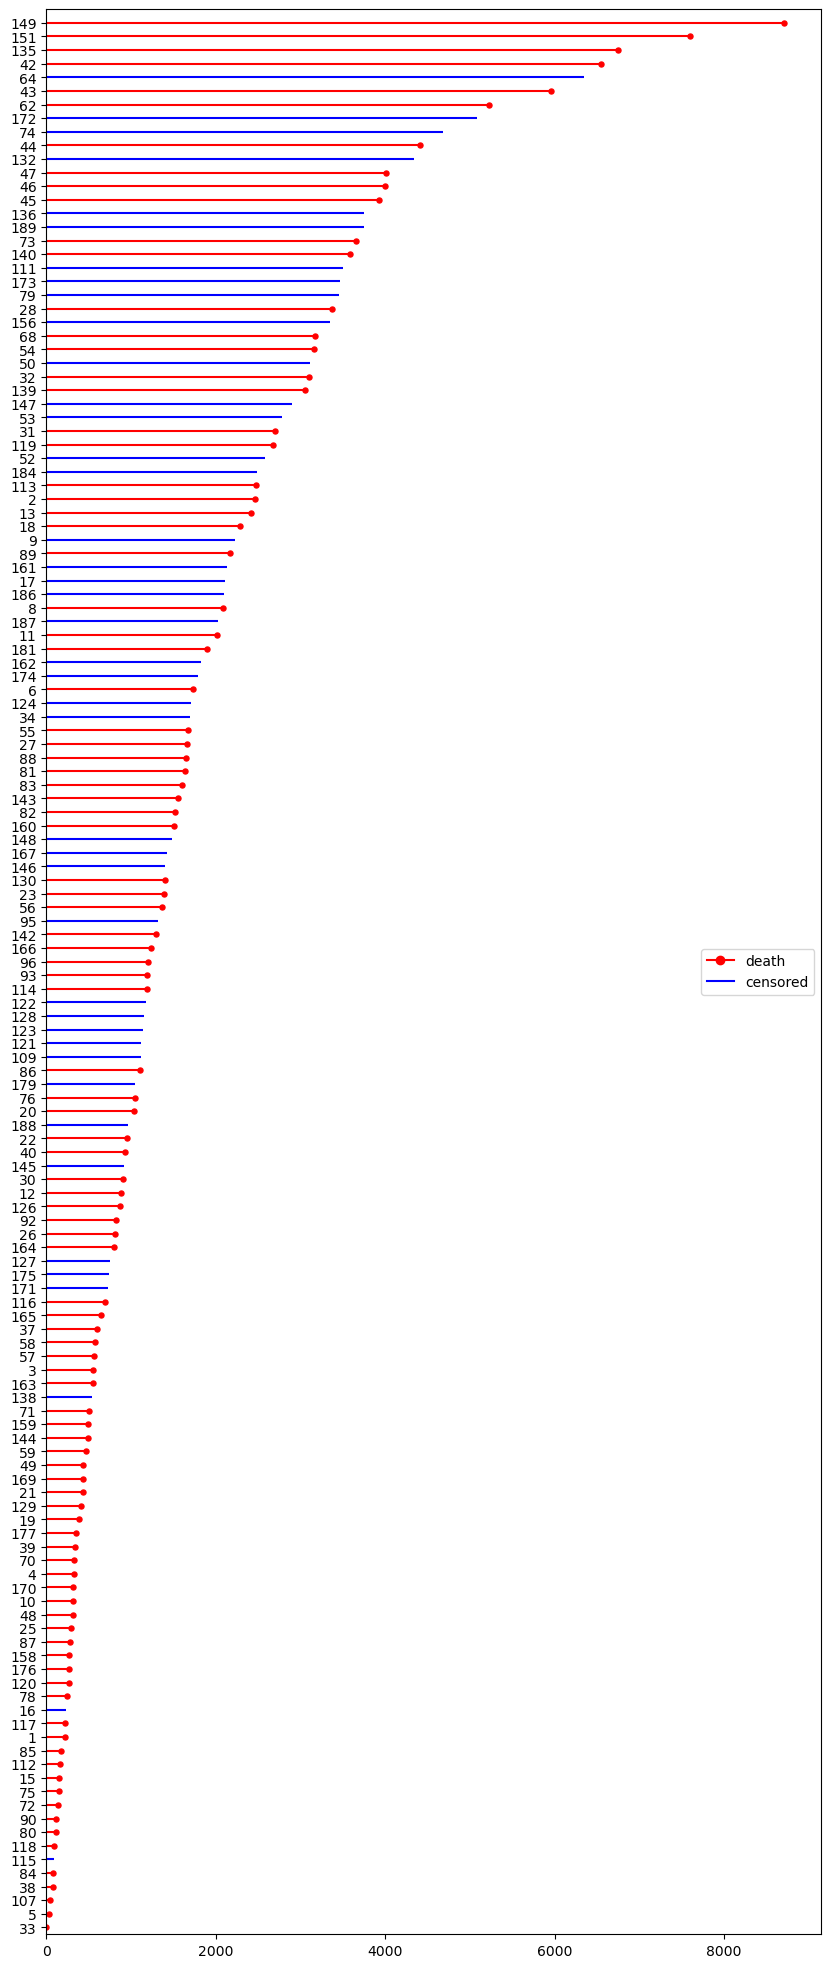
\includegraphics[height=0.71\pdfpageheight]{latex/figures/surv_race_full.png}
    \caption{Survival time of all patients in the cohort.}
    \label{fig:SurvRaceFull}
\end{figure}

\begin{figure}[H]
    \centering
     \begin{subfigure}[b]{0.49\textwidth}
         \centering
         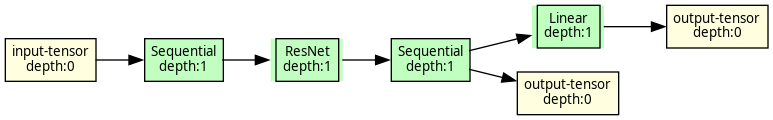
\includegraphics[width=\textwidth]{latex/networks/CosResNet.gv.png}
         \caption{ResNet}
     \end{subfigure}
    \hfill
     \begin{subfigure}[b]{0.49\textwidth}
         \centering
         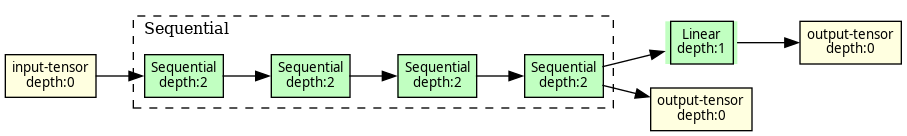
\includegraphics[width=\textwidth]{latex/networks/SNNet.gv.png}
         \caption{SNN}
     \end{subfigure}
\vskip\baselineskip
     \begin{subfigure}[b]{\textwidth}
         \centering
         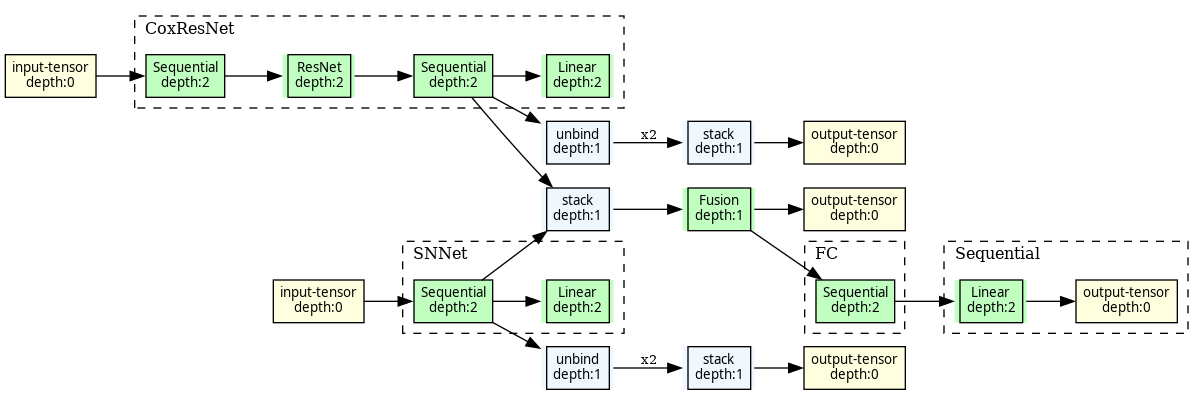
\includegraphics[width=\textwidth]{latex/networks/Mutlisurv.gv.png}
         \caption{Fusion Network of ResNet and SNN}
     \end{subfigure}
\vskip\baselineskip
     \begin{subfigure}[b]{\textwidth}
         \centering
         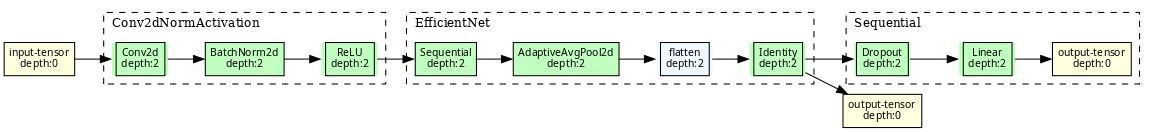
\includegraphics[width=\textwidth]{latex/networks/CoxEffNet.gv.png}
         \caption{EfficientNet}
     \end{subfigure}
% \vskip\baselineskip
%      \begin{subfigure}[b]{\textwidth}
%          \centering
%          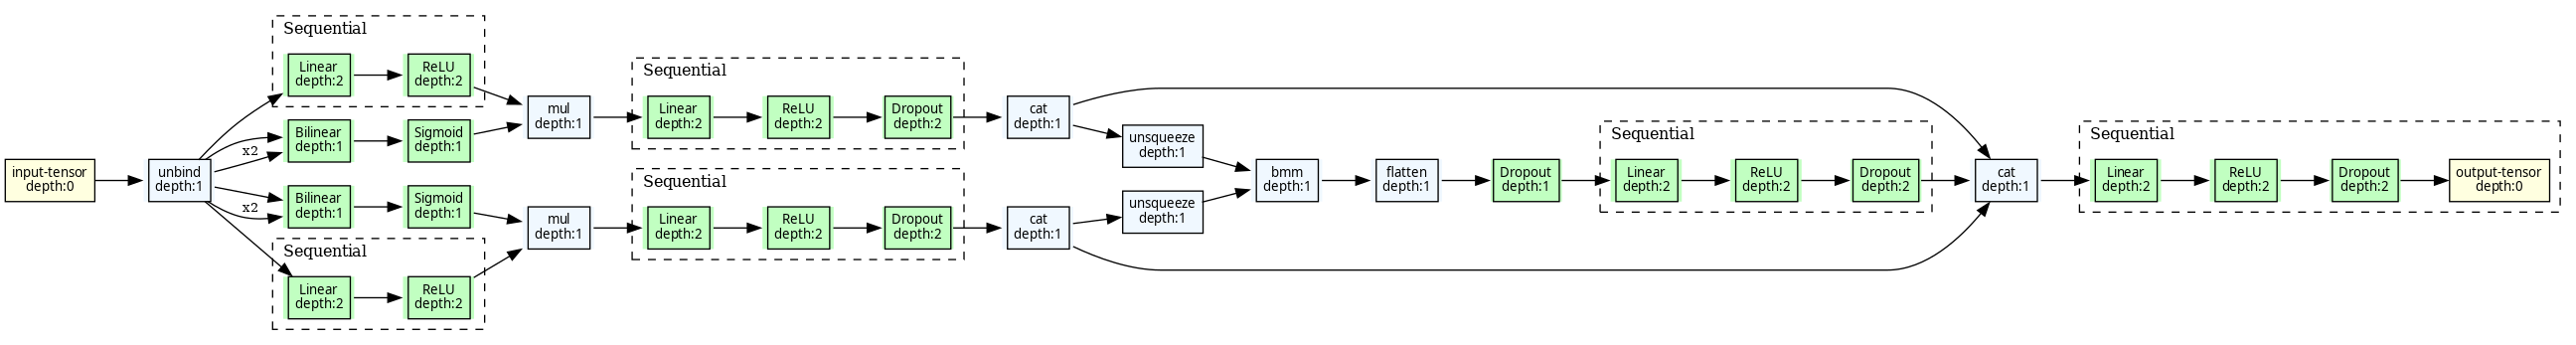
\includegraphics[width=\textwidth]{latex/networks/Kronecker.gv.png}
%          \caption{Saliency Maps}
%      \end{subfigure}
%     \hfill
    %  \begin{subfigure}[b]{0.49\textwidth}
    %      \centering
    %      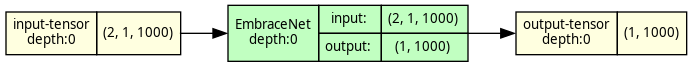
\includegraphics[width=\textwidth]{latex/networks/EmbraceNet.gv.png}
    %      \caption{Input*Gradient}
    %  \end{subfigure}
    % \hfill
    \caption[Network architectures]{Network architectures with varying level of detail. Each unimodal model returns a feature vector and the predicted hazard. Hence, the fusion network shows four terminal values. Graphs were generated using the Python package torchview. This visualisation reveals some minor implementation details that were not discussed in chapter \ref{MetMat}.}
    \label{fig:network_archs}
\end{figure}

\begin{figure}[H]
    \centering
     \begin{subfigure}[b]{0.475\textwidth}
         \centering
         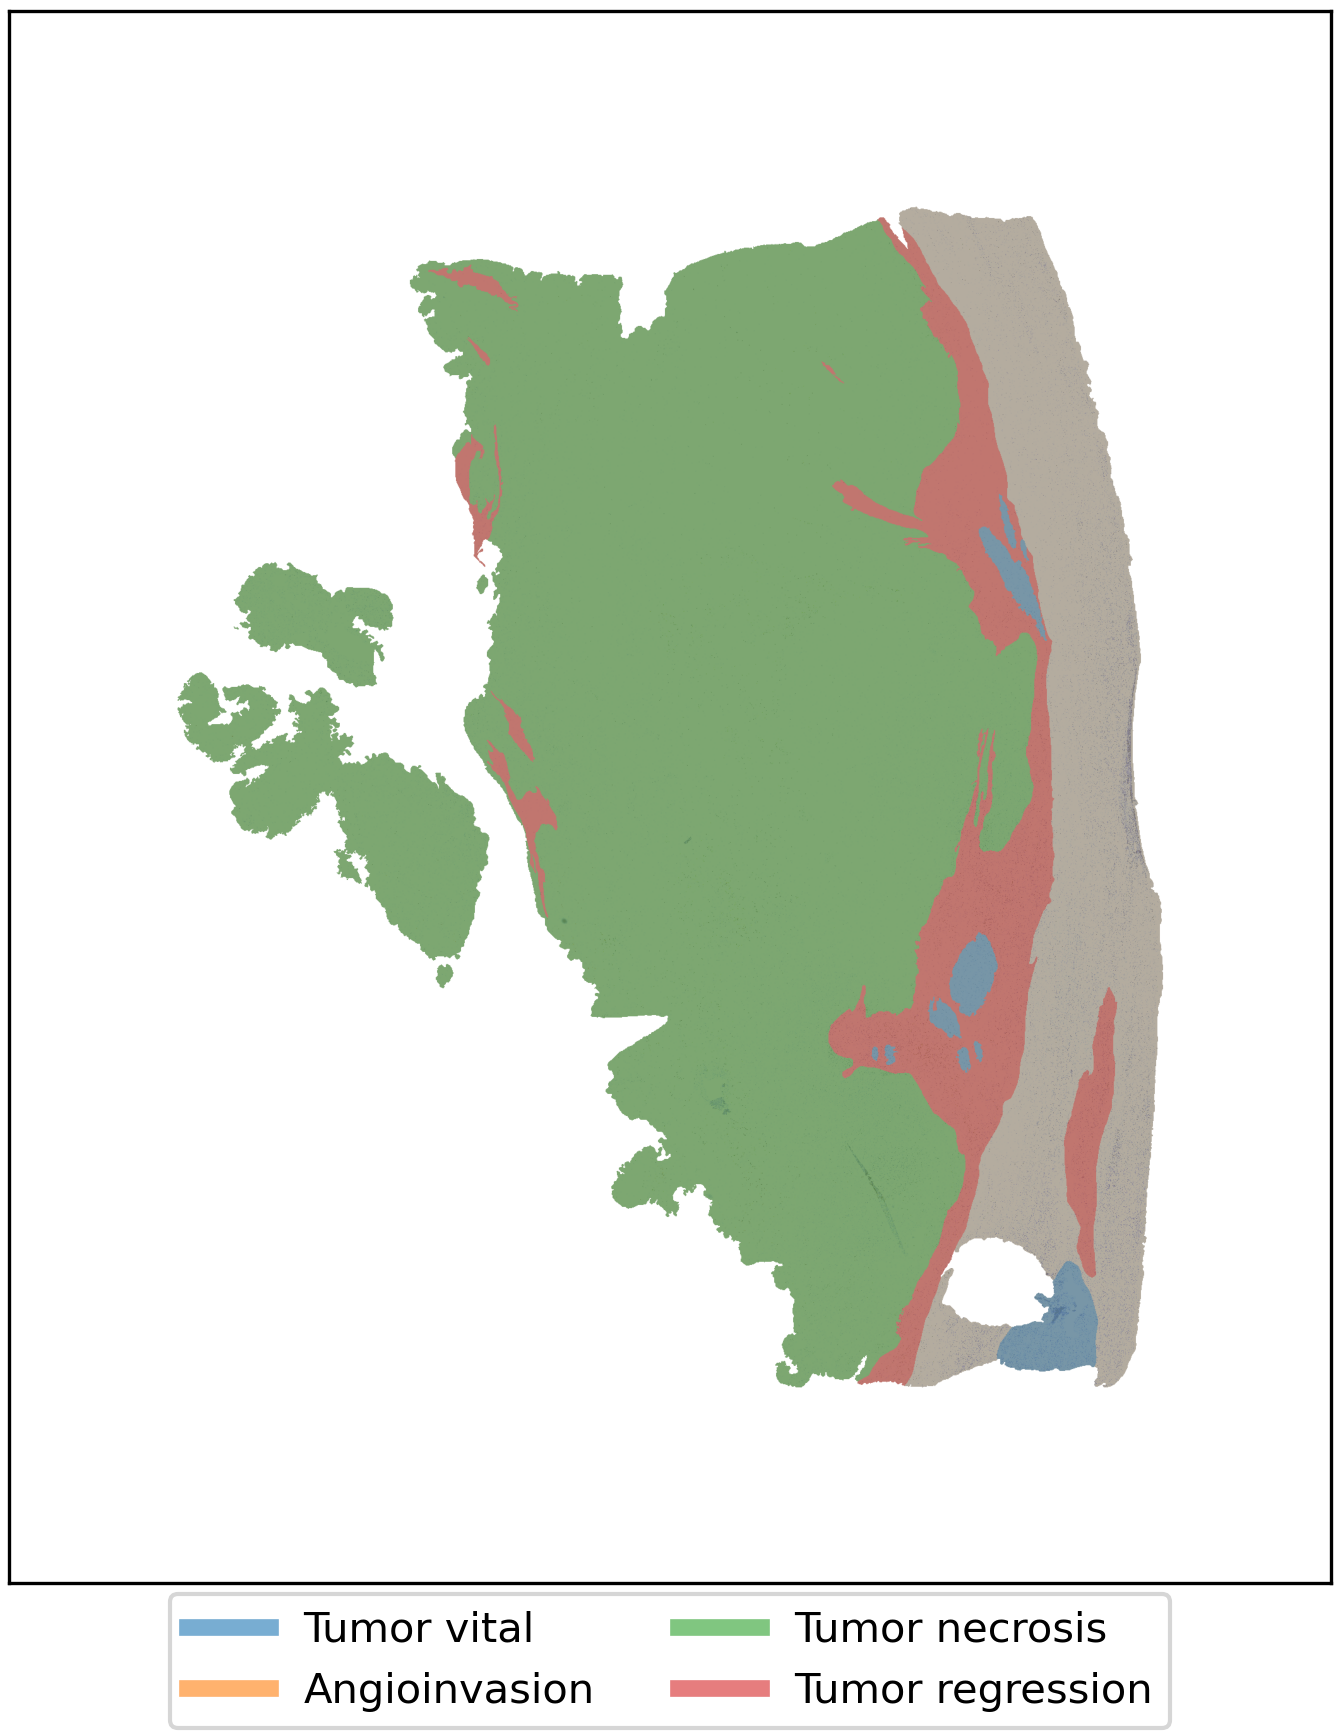
\includegraphics[width=\textwidth]{latex/captum/case121/masks_case121-stain19-censored_1119days.png}
         \caption{Tumour annotations of WSI}
     \end{subfigure}
    \hfill
     \begin{subfigure}[b]{0.49\textwidth}
         \centering
         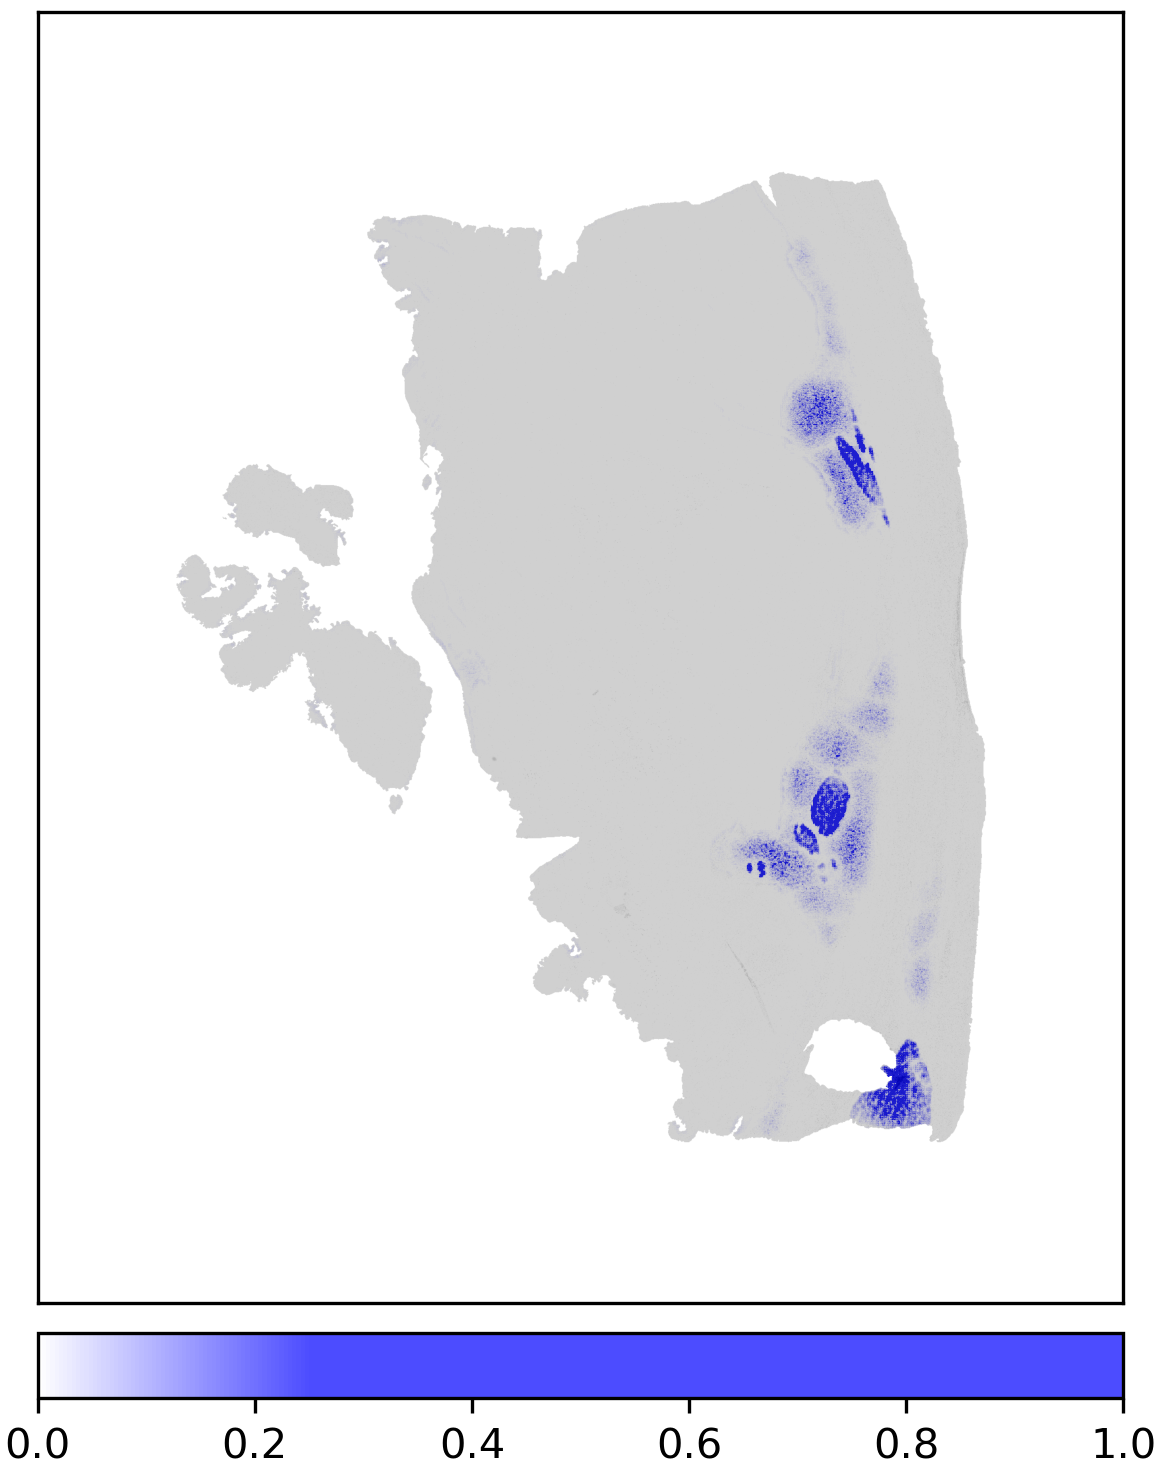
\includegraphics[width=\textwidth]{latex/captum/case121/integrated_gradients_abs_case121-stain19-censored_1119days.png}
         \caption{Integrated Gradients, abs. attributions}
     \end{subfigure}
\vskip\baselineskip
     \begin{subfigure}[b]{0.49\textwidth}
         \centering
         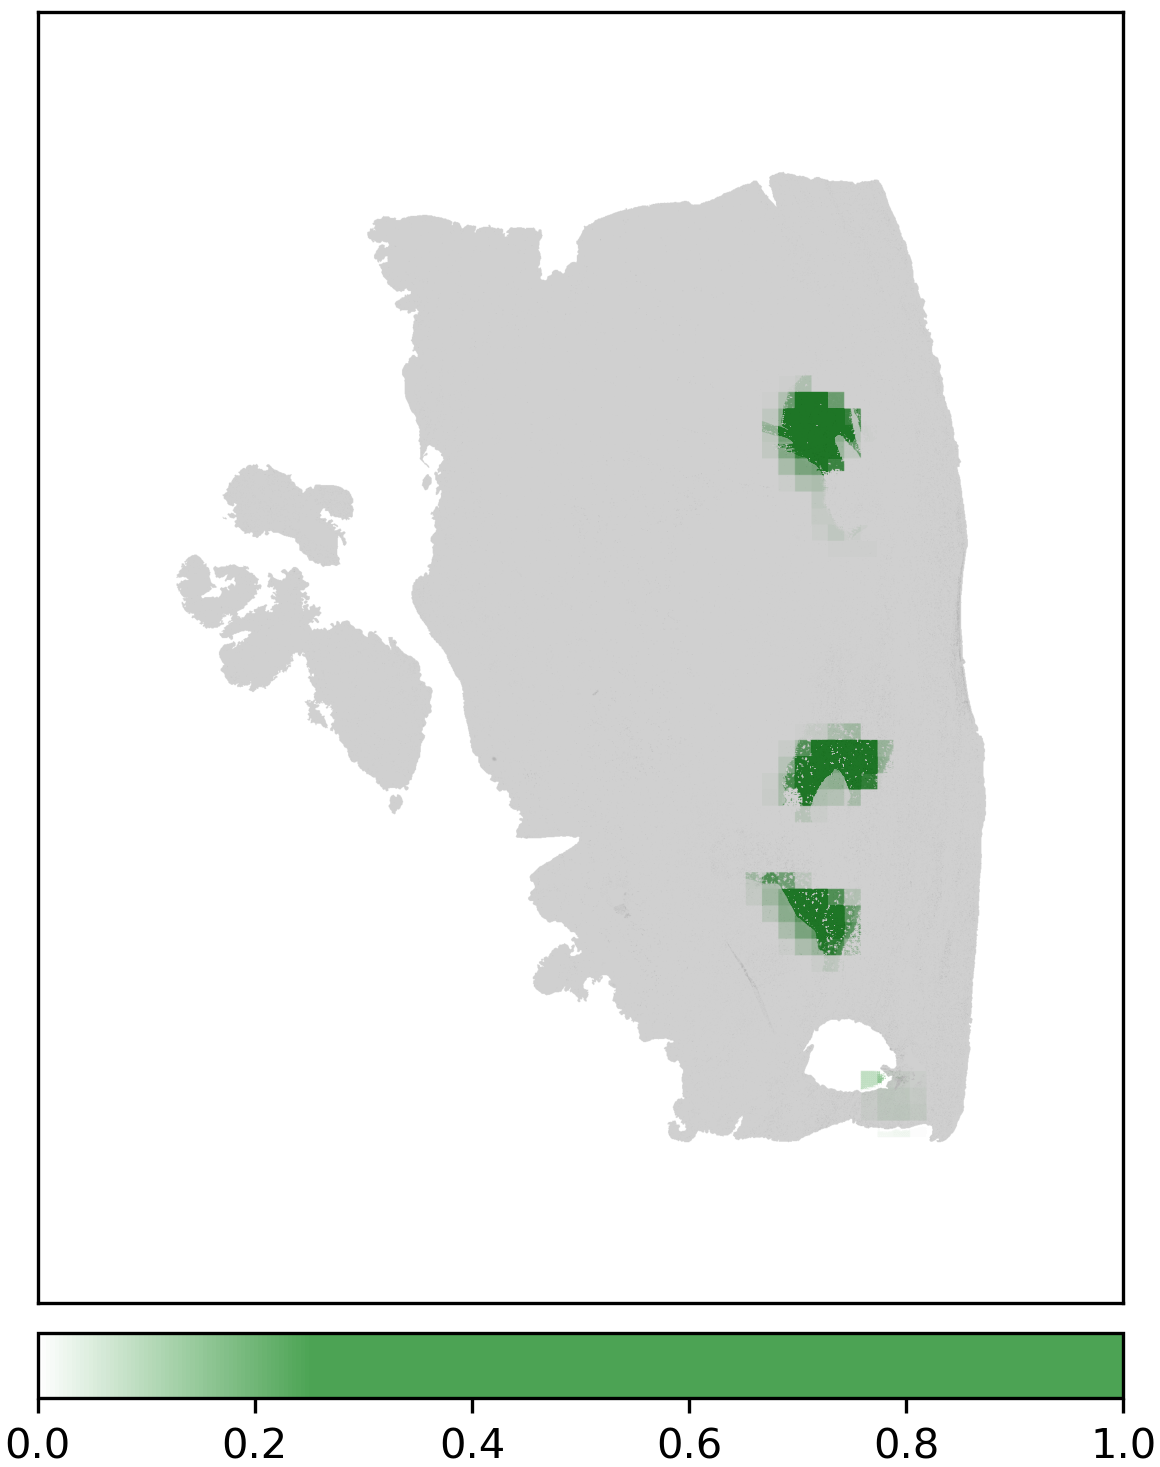
\includegraphics[width=\textwidth]{latex/captum/case121/guided_gradcam_pos_case121-stain19-censored_1119days.png}
         \caption{Guided GradCAM, positive attributions}
     \end{subfigure}
    \hfill
     \begin{subfigure}[b]{0.49\textwidth}
         \centering
         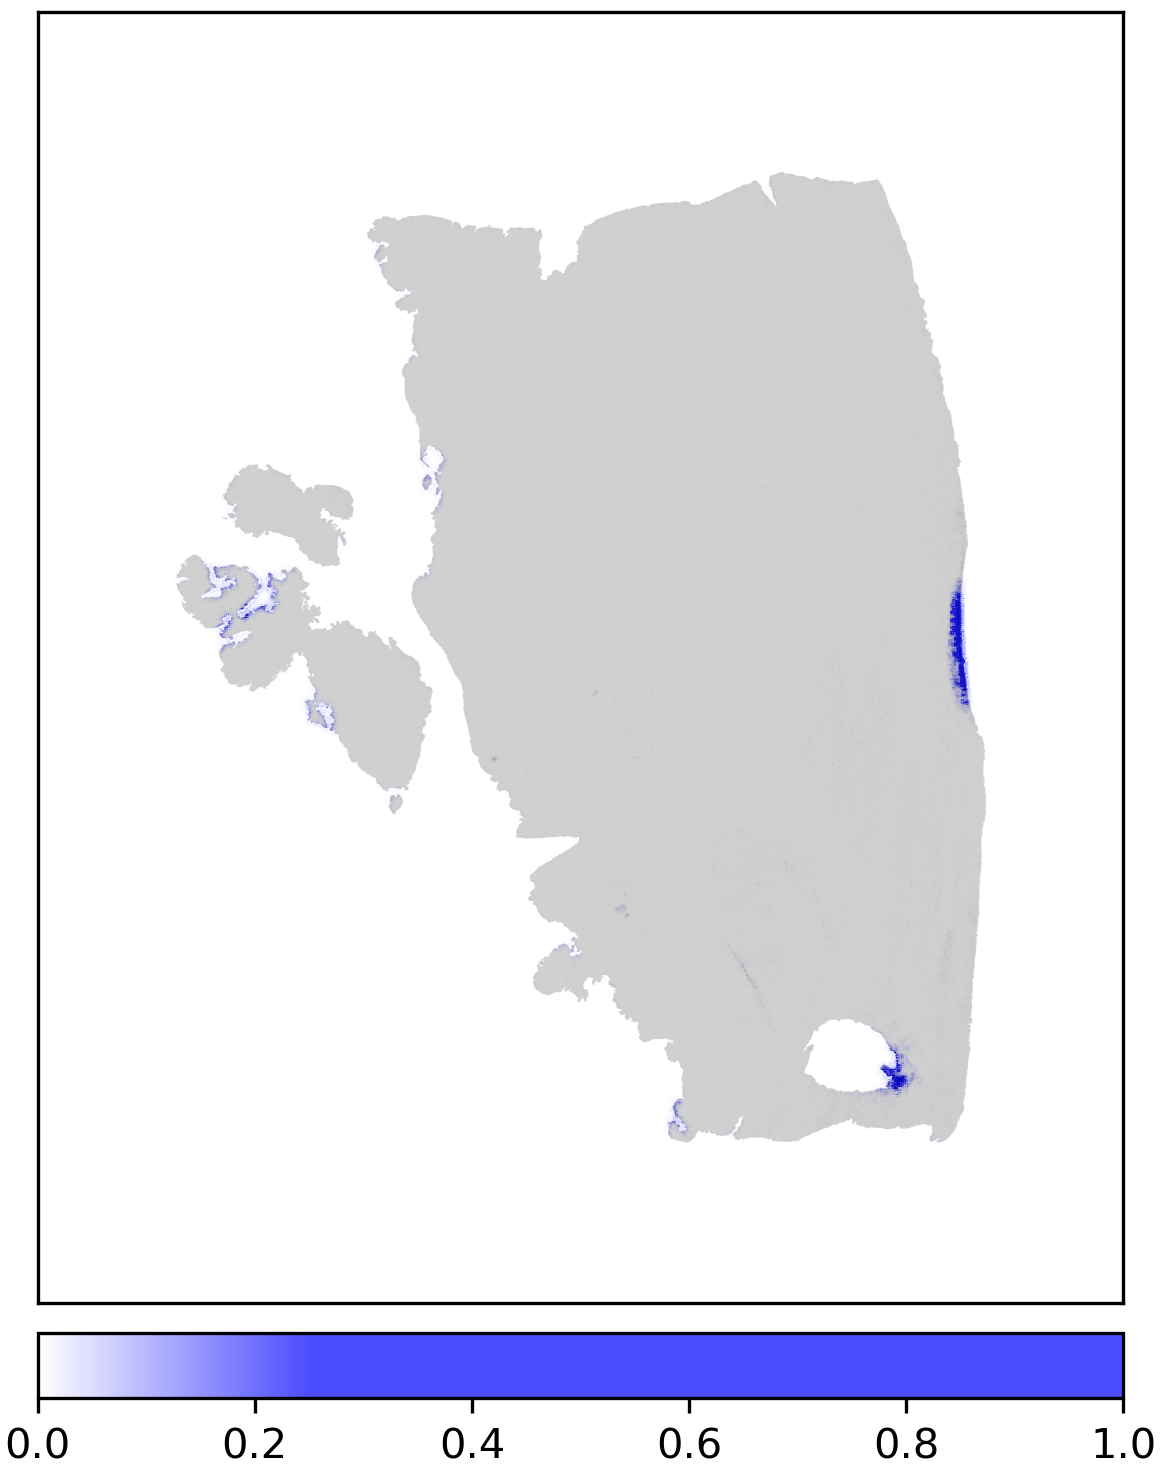
\includegraphics[width=\textwidth]{latex/captum/case121/saliency_case121-stain19-censored_1119days.png}
         \caption{Saliency Map, abs. attributions}
     \end{subfigure}
    \hfill
    \caption[Integrated gradients, Guided GradCAM and saliency for case 121 stain 19]{Results of Integrated Gradients and Guided GradCAM for case 121 stained for CD204. The figure of the tumour masks is included for comparison. Integrated Gradients and saliency attributions are converted to absolute values.}
    \label{fig:case121}
\end{figure}

\begin{figure}[H]
    \centering
     \begin{subfigure}[b]{0.475\textwidth}
         \centering
         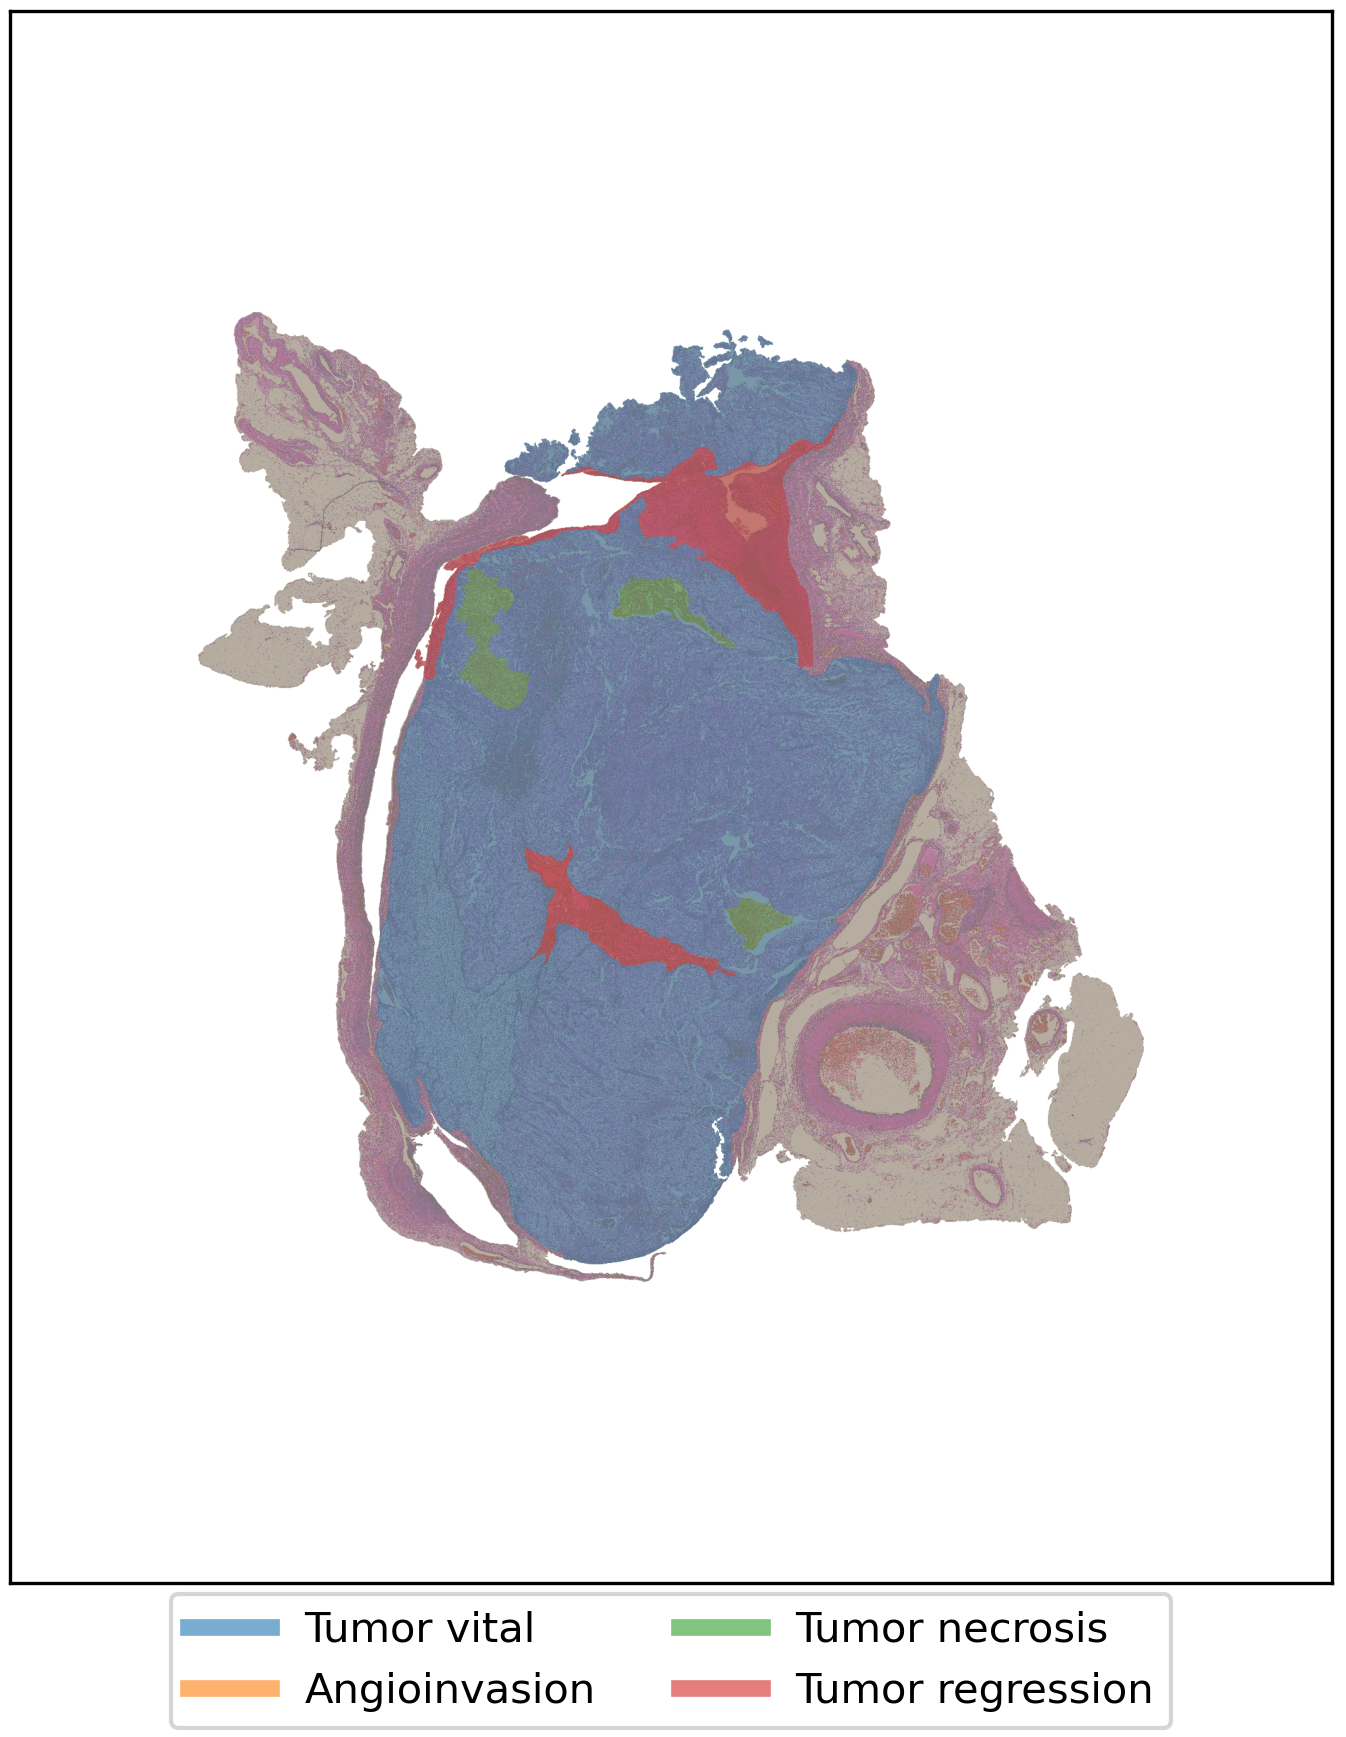
\includegraphics[width=\textwidth]{latex/captum/case181/masks_case181-stain1-dead_1893days.png}
         \caption{Tumour annotations of WSI}
     \end{subfigure}
    \hfill
     \begin{subfigure}[b]{0.49\textwidth}
         \centering
         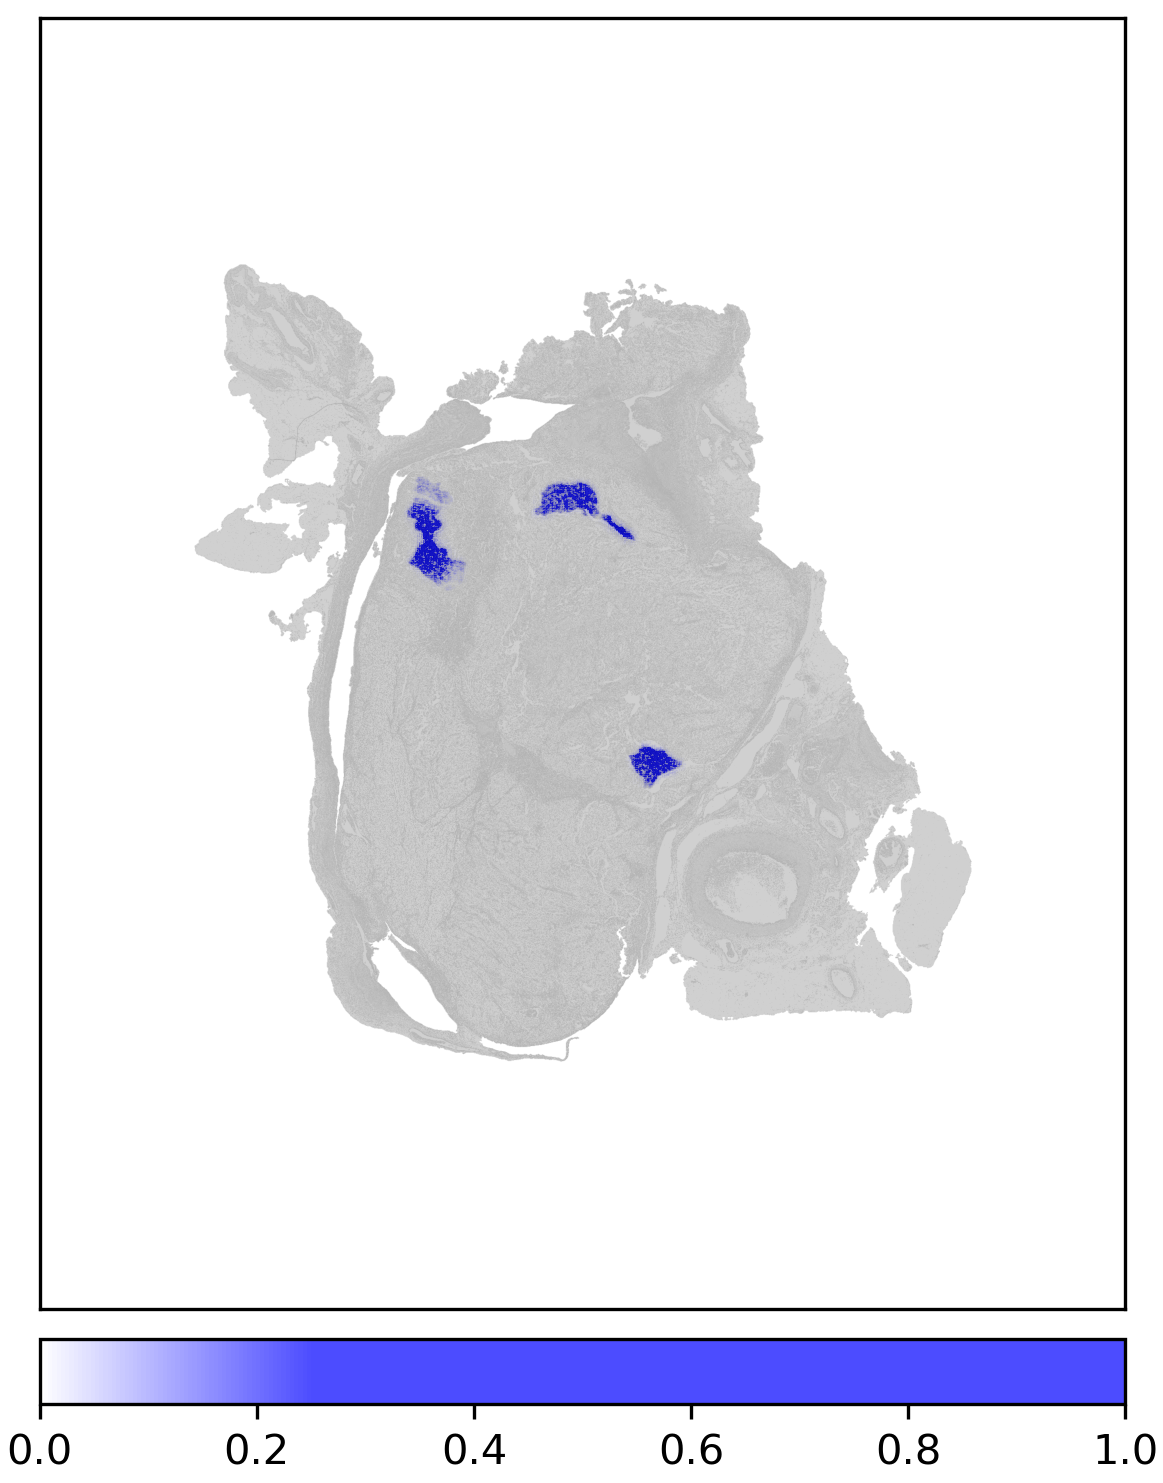
\includegraphics[width=\textwidth]{latex/captum/case181/integrated_gradients_abs_case181-stain1-dead_1893days.png}
         \caption{Integrated Gradients, abs. attributions}
     \end{subfigure}
\vskip\baselineskip
     \begin{subfigure}[b]{0.49\textwidth}
         \centering
         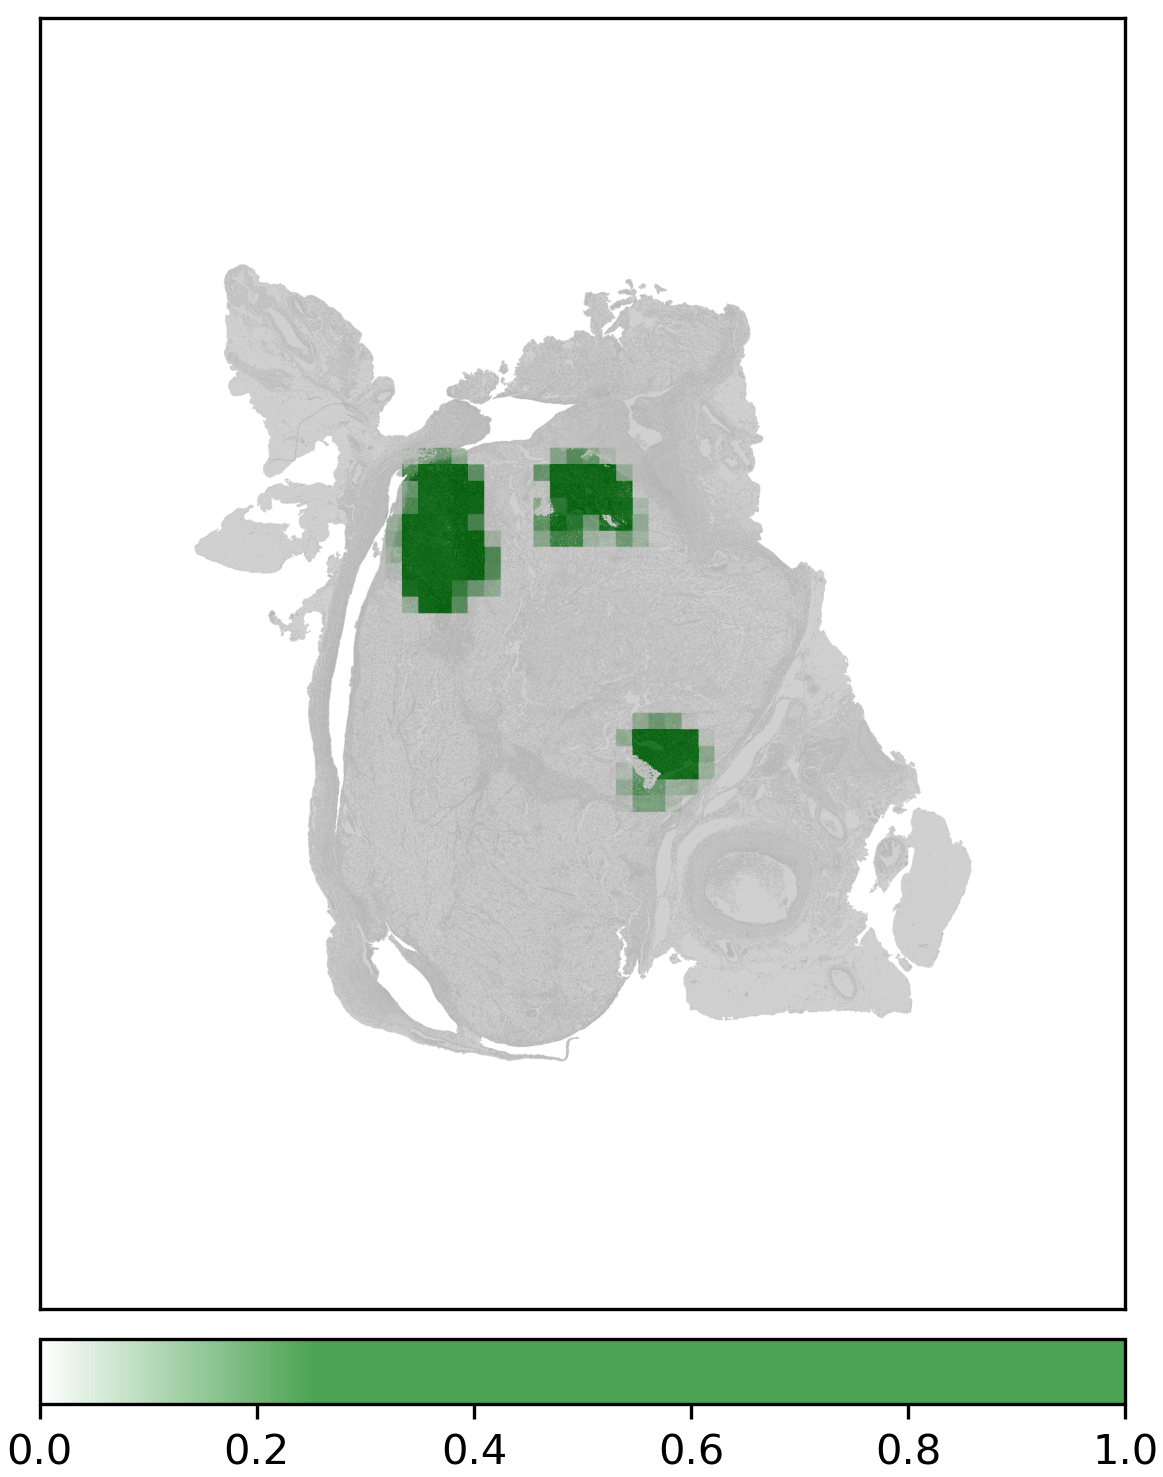
\includegraphics[width=\textwidth]{latex/captum/case181/guided_gradcam_pos_case181-stain1-dead_1893days.png}
         \caption{Guided GradCAM, positive attributions}
     \end{subfigure}
    \hfill
     \begin{subfigure}[b]{0.49\textwidth}
         \centering
         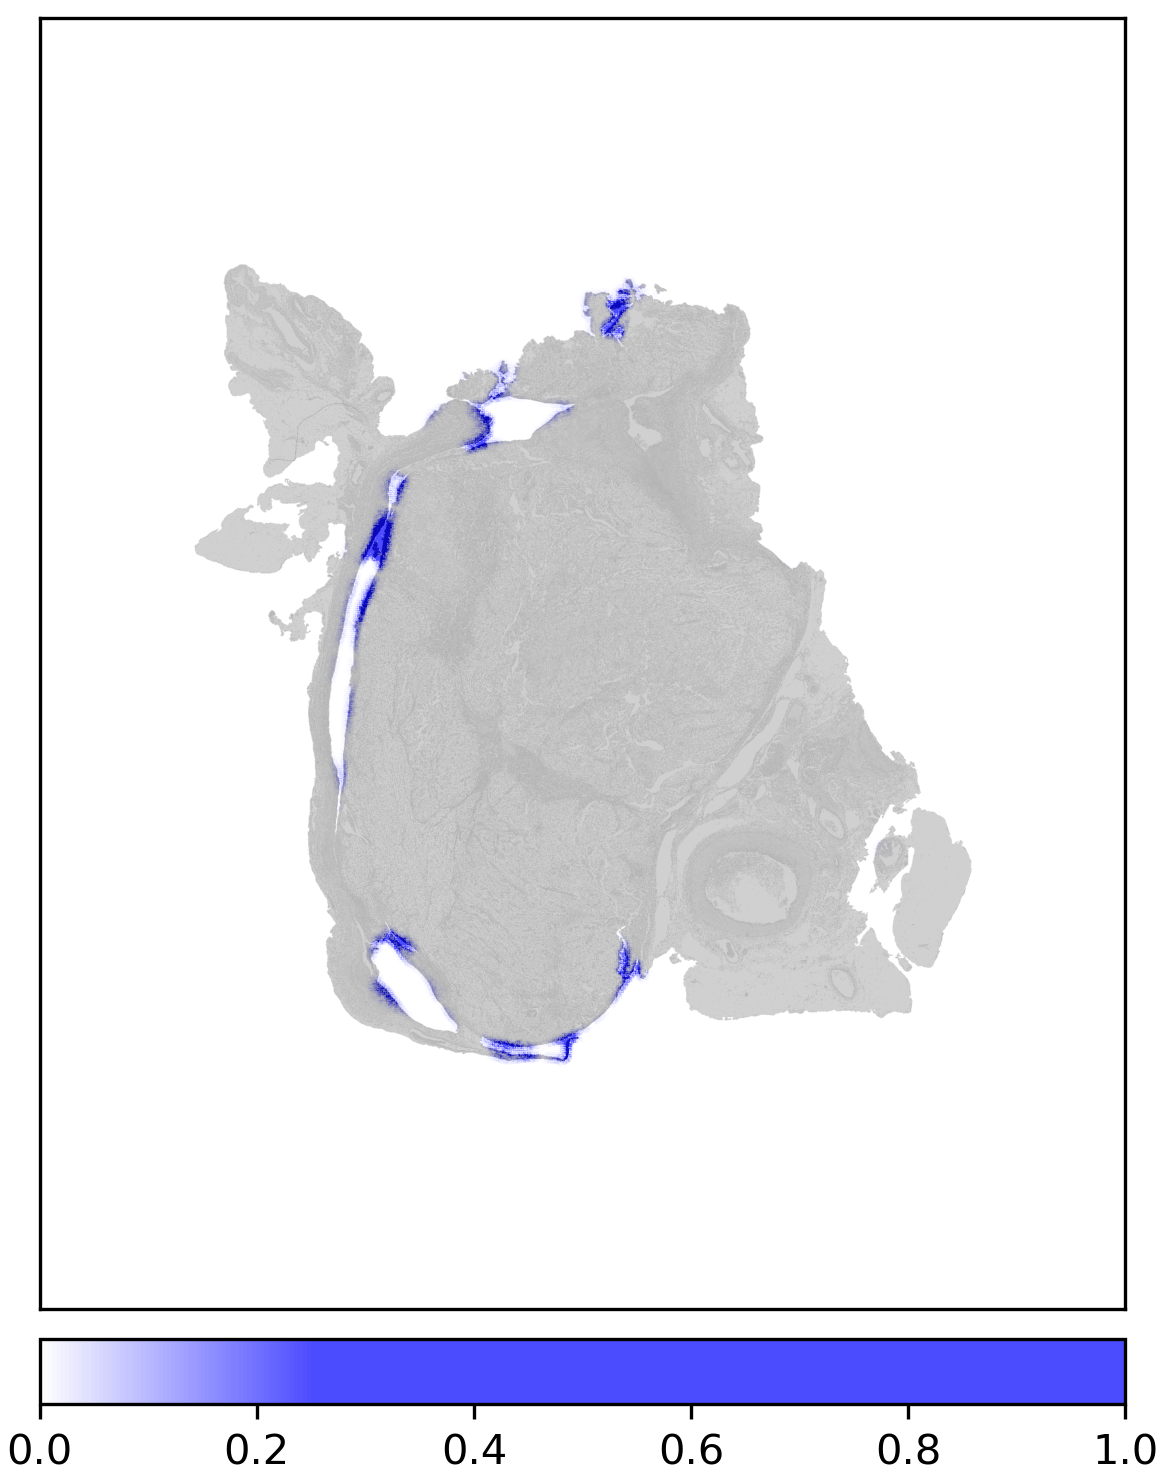
\includegraphics[width=\textwidth]{latex/captum/case181/saliency_case181-stain1-dead_1893days.png}
         \caption{Saliency Map, abs. attributions}
     \end{subfigure}
    \hfill
    \caption[Integrated gradients, Guided GradCAM and saliency for case 181 stain 1]{Results of Integrated Gradients and Guided GradCAM for case 181 stained with H\&E. The figure of the tumour masks is included for comparison. Integrated Gradients and saliency attributions are converted to absolute values.}
    \label{fig:case181}
\end{figure}